\documentclass[10pt]{article}
\usepackage[margin=0.8in]{geometry}
\usepackage[T1]{fontenc}
\usepackage{microtype,amsmath,amssymb,booktabs,graphicx,hyperref}
\usepackage[numbers]{natbib}
\graphicspath{{figures/}}
\title{STP-RAG: Semantic Transition Profiles for Adaptive Chunking and Selective Context}
\author{}
\date{}
\begin{document}
\maketitle
\begin{abstract}
We present a reference specification for retrieval-augmented question answering that combines adaptive passage boundaries based on local semantic transition profiles with budgeted selection of neighboring context, together with an unexecuted confirmatory protocol and an audited pilot. The specification is not a complete description of the pilot implementation. On HotpotQA, full STP with context has descriptive answer F1 of 0.410, compared with 0.358 for fixed-size chunking; on QASPER, fixed-size is best on all four reported quality metrics, and full-STP F1 decreases from 0.105 without context to 0.068 with context. Generation metrics use only 25 queries, and evidence alignment drops 42 of 149 QASPER questions. The nominal velocity-only arm also includes structural weighting, and chunking and prompt budgets are unmatched. These observations do not establish statistical significance, causal effects, or general superiority. A matched-budget, paired evaluation is proposed to test the individual design choices.
\end{abstract}
\section{Introduction}

Retrieval-augmented question answering depends on both finding evidence and making it usable by a reader. Early retrieve-and-read systems combined document search with answer extraction \cite{Chen2017ReadingWikipedia}, while learned retrievers and dense passage representations made retrieval a trainable component of open-domain QA \cite{Lee2019LatentRetrieval,Karpukhin2020DensePassage}. Retrieval-augmented language models extend this approach to pretraining and generation \cite{Guu2020RealmRetrievalaugmented,Lewis2020RetrievalaugmentedGeneration}, including settings that aggregate multiple passages or learn from few examples \cite{Izacard2020LeveragingPassage,Izacard2022FewshotLearning}. Surveys describe the resulting design space across retrieval, augmentation, generation, and evaluation \cite{Gao2023RetrievalaugmentedGeneration,Fan2024SurveyRag,Zhao2024RetrievalaugmentedGeneration,Yu2024EvaluationRetrievalaugmented}.

Two choices in this pipeline are how to divide source documents into retrieval units and how much surrounding text to supply after retrieval. Fixed-size passages are convenient, but a boundary can separate a definition from its qualification or place unrelated material together. Retrieval granularity has been shown to affect retrieval and downstream QA \cite{Chen2023DenseX}. Context also matters: performance can depend on where relevant material appears in a long prompt \cite{Liu2023LostMiddle}, and distracting information can degrade reasoning or reading comprehension \cite{Shi2023LargeLanguage,Jia2017AdversarialExamples}. These observations motivate studying segmentation and context selection together; they do not establish which boundaries or context policies are best for a particular dataset.

The supplied pilot considers two evidence-intensive settings. HotpotQA contains approximately 113,000 Wikipedia-based questions designed to require reasoning over multiple documents, with sentence-level supporting facts \cite{Yang2018HotpotqaDataset}. QASPER contains 5,049 information-seeking questions over 1,585 research papers, with answers and supporting evidence anchored in the full text \cite{Dasigi2021DatasetInformationseeking}. These settings make evidence coverage and provenance important, as also reflected in knowledge-intensive evaluation that assesses both task outputs and provenance \cite{Petroni2020KiltBenchmark}. Sentence representations suitable for similarity comparisons provide one possible basis for measuring local changes in meaning \cite{Reimers2019SentencebertSentence}.

We propose STP-RAG, a reference specification that uses a \emph{semantic transition profile} to investigate adaptive boundaries and selective context. Ordered sentence units retain source offsets and structural metadata. A boundary score combines adjacent embedding distance, positive acceleration in that distance, trailing-window volatility, and structural indicators, with development-only robust normalization and length constraints. After retrieval, nearby source units are ranked using relevance, structural affinity, reference or entity overlap, and distance, and are attached within a declared token budget while retaining provenance. This specification should be distinguished from the audited pilot implementation and from the unexecuted confirmatory protocol.

The pilot findings are mixed and descriptive. On HotpotQA, answer F1 is 0.410 for full STP with context, compared with 0.358 for fixed-size chunking and 0.344 for the nominal velocity arm; that arm actually computes velocity with structural weighting. It has the strongest reported HotpotQA Recall@5 and MRR among the pilot arms. On QASPER, fixed-size chunking is best on all four reported quality metrics, and full-STP answer F1 falls from 0.105 without context to 0.068 with context. Generation metrics use only 25 queries, and evidence alignment drops 42 of 149 QASPER questions. Arms differ in indexed material, chunk counts, and prompt volume: audit estimates for the top-three-chunk prompts are roughly 960 evidence tokens for fixed-size, 345 for full STP without context, and 945 for full STP with context. Thus the HotpotQA context difference is consistent with restored prompt volume and cannot be attributed to selection quality. The aggregates do not establish causal effects, statistical significance, or general superiority.

This paper contributes (1) an explicit transition-profile and provenance-preserving context-selection specification, (2) an audited account of mixed pilot results, and (3) a confirmatory protocol with paired per-query records, matched chunk-length distributions and prompt budgets, intrinsic segmentation and context diagnostics, and document-clustered inference. The protocol is a proposed evaluation, not a completed benchmark.

\section{Related Work}

\subsection{Fixed and Similarity-Based Segmentation}

Text segmentation has long sought boundaries that produce coherent contiguous units. Choi uses locally ranked sentence similarities and divisive clustering \cite{Choi2000AdvancesDomain}; embedding-based approaches include segmentation objectives based on word vectors \cite{Alemi2015TextSegmentation} and semantic-relatedness graphs whose cliques define segments \cite{Glavas2016UnsupervisedText}. Probabilistic alternatives optimize a statistical segmentation model \cite{Utiyama2001StatisticalModel} or model lexical cohesion and discourse cues in a Bayesian framework \cite{Eisenstein2008BayesianUnsupervised}. These approaches motivate semantic boundaries but address segmentation settings that need not coincide with retrieval-oriented chunking.

Recent RAG studies examine chunking as part of a broader system. Qu et al.\ report that semantic chunking's extra computational cost does not yield consistent gains over fixed-size chunking across their retrieval-related tasks \cite{Qu2024SemanticChunking}; Wang et al.\ investigate combinations of RAG design choices and their performance--efficiency trade-offs \cite{Wang2024SearchingBest}. Our pilot includes a fixed-size arm, whereas a similarity-threshold arm is only planned for the confirmatory study. The reference STP score differs conceptually from a single similarity threshold by combining multiple local signals with length constraints; its benefit over that proposed baseline has not been measured.

\subsection{Transition- and Structure-Aware Segmentation}

Supervised segmentation can learn boundary decisions from labeled examples \cite{Koshorek2018TextSegmentation}, while SECTOR learns topic representations for section segmentation and classification \cite{Arnold2019SectorNeural}. Other methods consider context beyond an adjacent pair: a graph-cut model incorporates long-range cohesion in lecture segmentation \cite{Malioutov2006MinimumCut}, and cross-segment attention uses transformer architectures for segmentation \cite{Lukasik2020TextSegmentation}. Such approaches provide alternatives to a scalar local transition score rather than evaluated competitors in our pilot.

STP-RAG instead specifies an interpretable combination of velocity, positive acceleration, volatility, and structural indicators. Structure and semantic change may disagree, and no single cue is assumed to capture every useful boundary. Segmentation similarity and annotator-agreement measures explicitly address variation in boundary placement \cite{Fournier2012SegmentationSimilarity}. The planned protocol complements downstream QA with intrinsic segmentation metrics and evidence-split rate. In the pilot, the nominal velocity-only arm retains structural weighting, so it is more accurately described as velocity plus structure. Clean velocity-only, structure-only, and other component ablations remain planned.

\subsection{Selective Context and Retrieval}

Context can be controlled at several stages. LongRAG enlarges retrieval units and uses a long-context reader \cite{Jiang2024LongragEnhancing}; RAPTOR retrieves from a hierarchy of chunks and recursive summaries \cite{Sarthi2024RaptorRecursive}. Late chunking instead incorporates surrounding document context into chunk embeddings before pooling \cite{Gunther2024LateChunking}. These approaches differ from attaching selected neighboring source units after retrieval. Comparisons of RAG with long-context models also highlight a quality--cost trade-off \cite{Li2024RetrievalAugmented}; LongBench and RULER offer complementary tests of long-context understanding and its dependence on task complexity and length \cite{Bai2023LongbenchBilingual,Hsieh2024RulerWhats}.

Selection and compression provide further alternatives to unrestricted expansion. RECOMP uses extractive or abstractive compression and can omit unhelpful augmentation \cite{Xu2023RecompImproving}; LLMLingua and LongLLMLingua compress prompts to manage token budgets \cite{Jiang2023LlmlinguaCompressing,Jiang2023LongllmlinguaAccelerating}. RankRAG trains a model for both context ranking and generation \cite{Yu2024RankragUnifying}, while Chain-of-Note generates notes to assess and synthesize retrieved documents \cite{Yu2023ChainofnoteEnhancing}. The STP-RAG reference design ranks nearby source units and preserves their provenance rather than generating summaries. Relevance-only and profile-guided context policies are proposed comparisons, not completed pilot arms.

Adaptive retrieval can also gather evidence over multiple steps. Multi-hop dense retrieval, condensed retrieval, and interleaved reasoning and retrieval address questions whose evidence must be assembled across passages \cite{Xiong2020AnsweringComplex,Khattab2021BaleenRobust,Trivedi2022InterleavingRetrieval}; MuSiQue provides a benchmark constructed to require connected multi-hop reasoning \cite{Trivedi2021MusiqueMultihop}. Self-RAG and active retrieval study when to retrieve or use evidence during generation \cite{Asai2023SelfragLearning,Jiang2023ActiveRetrieval}. These methods address retrieval and generation control at a different level from the proposed local boundary and neighbor-selection signals; the pilot does not compare against them.

\subsection{Evaluation and System Trade-offs}

Retrieval and answer quality need separate measurement. SQuAD provides a widely used reading-comprehension setting with answer-span evaluation \cite{Rajpurkar2016Squad100000}, while RAGChecker proposes fine-grained diagnostics for retrieval and generation \cite{Ru2024RagcheckerFinegrained}. The confirmatory protocol accordingly plans retrieval, answer, segmentation, and context metrics with paired records and matched budgets. This is especially important here because the pilot changes both chunking and the volume of evidence supplied to the generator.

Operational measurements also depend on indexing and search choices. ANN-Benchmarks evaluates approximate nearest-neighbor quality and performance trade-offs \cite{Aumller2018AnnbenchmarksBenchmarking}, and work on large-scale similarity search examines indexing and search efficiency \cite{Johnson2017BillionscaleSimilarity}. Surveys of dense retrieval, transformer ranking, and language models for information retrieval describe further choices in representation, indexing, reranking, and readers \cite{Zhao2022DenseText,Yates2020PretrainedTransformers,Zhu2023LargeLanguage}. Because the pilot omits the retrieval backend, hardware, and timing boundaries, its retrieval latencies cannot establish end-to-end deployment speed.

\section{Method}

\subsection{Document Units and Transition Profiles}

We describe a reference design, not a verified account of every operation in the pilot. Let a document consist of ordered sentence units $u_1,\ldots,u_n$, each associated with source offsets and available structural metadata. A fixed encoder maps each unit to an L2-normalized embedding $e_i$. For the candidate boundary between $u_i$ and $u_{i+1}$, semantic velocity is the adjacent embedding distance
\[
v_i=d(e_i,e_{i+1}).
\]
The exact distance function is unspecified. Positive acceleration is the increase in velocity,
\[
a_i=\max\{0,v_i-v_{i-1}\},
\]
where the preceding velocity is available. A trailing-window volatility feature summarizes variation in recent velocities, and structural indicators record cues such as heading or paragraph changes. The window definition, its handling at document edges, and the detailed structural processing remain unspecified.

Continuous features are normalized using medians and interquartile ranges estimated on development data only. A weighted boundary score combines the normalized transition features and structural indicators. Boundary selection is subject to minimum, target, and maximum chunk-length constraints. The reference does not prescribe numerical weights, thresholds, a particular selection algorithm, or constraint values. These choices must be declared before a reproducible implementation can be evaluated.

\subsection{Selective Context and Provenance}

After retrieval, the reference design ranks nearby source units using embedding relevance, structural affinity, reference or entity overlap, and distance. It appends selected units within a declared context-token budget. The ranking equation, candidate neighborhood, and tie-breaking rule are not specified. Each indexed chunk and attached unit retains source provenance, including its document and offsets, so that selected evidence can be traced back to the source.

The pilot distinguishes full STP with and without context, but the available audit does not establish that all details of this reference design were implemented. In particular, it does not supply the exact structural processing or calibrated weights. The context comparison should therefore be interpreted as a comparison of recorded pilot conditions, not as a verification of the specification.

\section{Pilot Study and Confirmatory Protocol}

\subsection{Pilot Setup and Audit}

The pilot reports aggregate results for HotpotQA and QASPER under fixed-size chunking, a nominal velocity-only condition, and full STP, including a selective-context condition. The nominal velocity-only condition retains a structural weight; we call its computation \emph{velocity + structure}. It is not a clean test of velocity alone. Generation metrics use only 25 queries. For QASPER, evidence alignment drops 42 of 149 questions.

Every arm passes its top three chunks to the generator, but equal chunk counts do not imply equal evidence budgets. Fixed-size chunks average approximately 300--350 tokens, whereas full-STP chunks average approximately 95--121 tokens. The audit estimates in Table~\ref{tab:volume} are derived from mean chunk lengths, not measured per-query prompt counts. Arms also differ in chunk counts, indexed material, and context attachment behavior. These differences limit comparisons of both retrieval and generation.

\begin{table}[t]
\centering
\begin{tabular}{lr}
\toprule
Condition & Estimated evidence tokens \\
\midrule
Fixed-size & $\sim 960$ \\
Full STP without context & $\sim 345$ \\
Full STP with context & $\sim 945$ \\
\bottomrule
\end{tabular}
\caption{Audit estimates of generator evidence volume for the top-three-chunk prompts. Estimates are derived from mean chunk lengths, not per-query token counts.}
\label{tab:volume}
\end{table}

\subsection{Descriptive Pilot Results}

Table~\ref{tab:results} reports the supplied numerical quality aggregates. On HotpotQA, full STP with context has answer F1 of 0.410, versus 0.344 for velocity + structure and 0.358 for fixed-size. The respective differences, 0.066 and 0.052, are descriptive rather than tests or causal effects. Velocity + structure has the strongest reported HotpotQA Recall@5 and MRR, so the answer-F1 ordering does not extend to every retrieval metric.

\begin{table}[t]
\centering
\begin{tabular}{llr}
\toprule
Dataset & Condition and metric & Mean \\
\midrule
HotpotQA & Fixed-size, answer F1 & 0.358 \\
HotpotQA & Velocity + structure, answer F1 & 0.344 \\
HotpotQA & Full STP with context, answer F1 & 0.410 \\
\midrule
QASPER & Fixed-size, Recall@5 & 0.379 \\
QASPER & Velocity + structure, Recall@5 & 0.252 \\
QASPER & Full STP, Recall@5 & 0.299 \\
QASPER & Full STP without context, answer F1 & 0.105 \\
QASPER & Full STP with context, answer F1 & 0.068 \\
\bottomrule
\end{tabular}
\caption{Descriptive pilot aggregates. Generation metrics use 25 queries. The context condition for the reported QASPER Recall@5 values is not specified in the ledger.}
\label{tab:results}
\end{table}

On QASPER, fixed-size is best on all four reported quality metrics. Its Recall@5 is 0.379, compared with 0.299 for full STP and 0.252 for velocity + structure. Full STP is thus 21.1\% below fixed-size on this reported recall measure. Full-STP answer F1 decreases from 0.105 without context to 0.068 with context. The supplied aggregates do not identify whether retrieval coverage, the content or volume of attached context, or other differences account for these patterns.

The context comparison is particularly confounded: the estimated evidence volume for full STP with context is close to that of fixed-size, while the estimate without context is substantially smaller. Restored prompt volume is consistent with the observed HotpotQA context gain, but it prevents attribution of that gain to selection quality. Conversely, the QASPER decrease does not establish that adding context itself causes harm under a matched budget. No paired confidence intervals or hypothesis tests are available.

The reported mean QASPER chunk count is 47.959 for full STP and 41.796 for velocity + structure. More chunks do not demonstrate better section preservation. Figure~\ref{fig:structure} displays the supplied descriptive relationship between chunk count and F1; the two datasets and conditions do not exhibit a single common ordering. Figure~\ref{fig:delta} shows rounded differences against the nominal velocity baseline, including a positive HotpotQA F1 difference for STP with context and a negative QASPER difference. Neither plot isolates individual transition features.

The ledger reports a largest mean retrieval latency of 3.972\,ms, but the supplied latency figure displays QASPER means above 7\,ms. This discrepancy cannot be resolved from the available records. Figure~\ref{fig:latency} is therefore included as an unverified descriptive asset, not as evidence for a maximum latency or a deployment trade-off. Its error bars are across-seed standard deviations, not paired confidence intervals. Timing boundaries and caching are undocumented, and retrieval timing is not end-to-end latency.

The supplied figures also display labels for similarity and velocity-plus-acceleration conditions, but the evidence ledger does not provide their underlying numerical results or sufficient implementation details. We do not treat those plotted labels as verified empirical comparisons; the similarity-threshold baseline in the protocol below remains planned.

\begin{figure}[t]
\centering
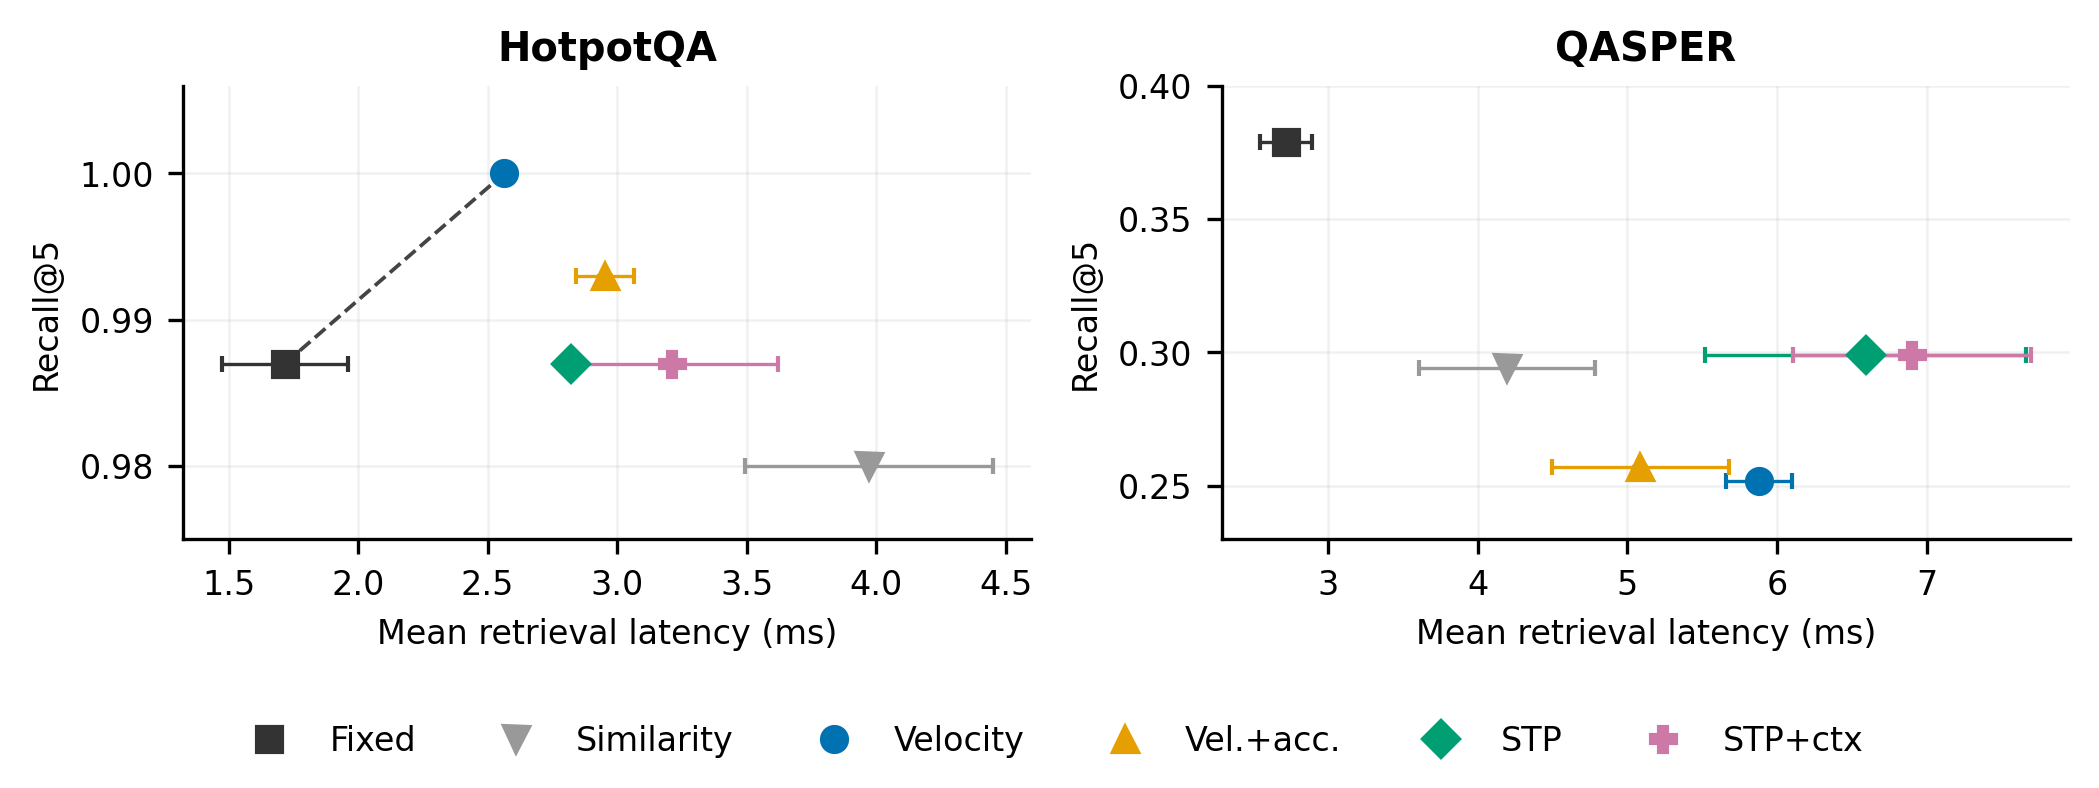
\includegraphics[width=\textwidth]{pareto_latency_recall.png}
\caption{Supplied descriptive Recall@5 versus mean retrieval latency plot. Horizontal error bars are across-seed standard deviations, not paired confidence intervals. The QASPER timing scale conflicts with the ledger's reported largest mean latency; plotted conditions beyond those documented in the ledger are not verified comparisons.}
\label{fig:latency}
\end{figure}

\begin{figure}[t]
\centering
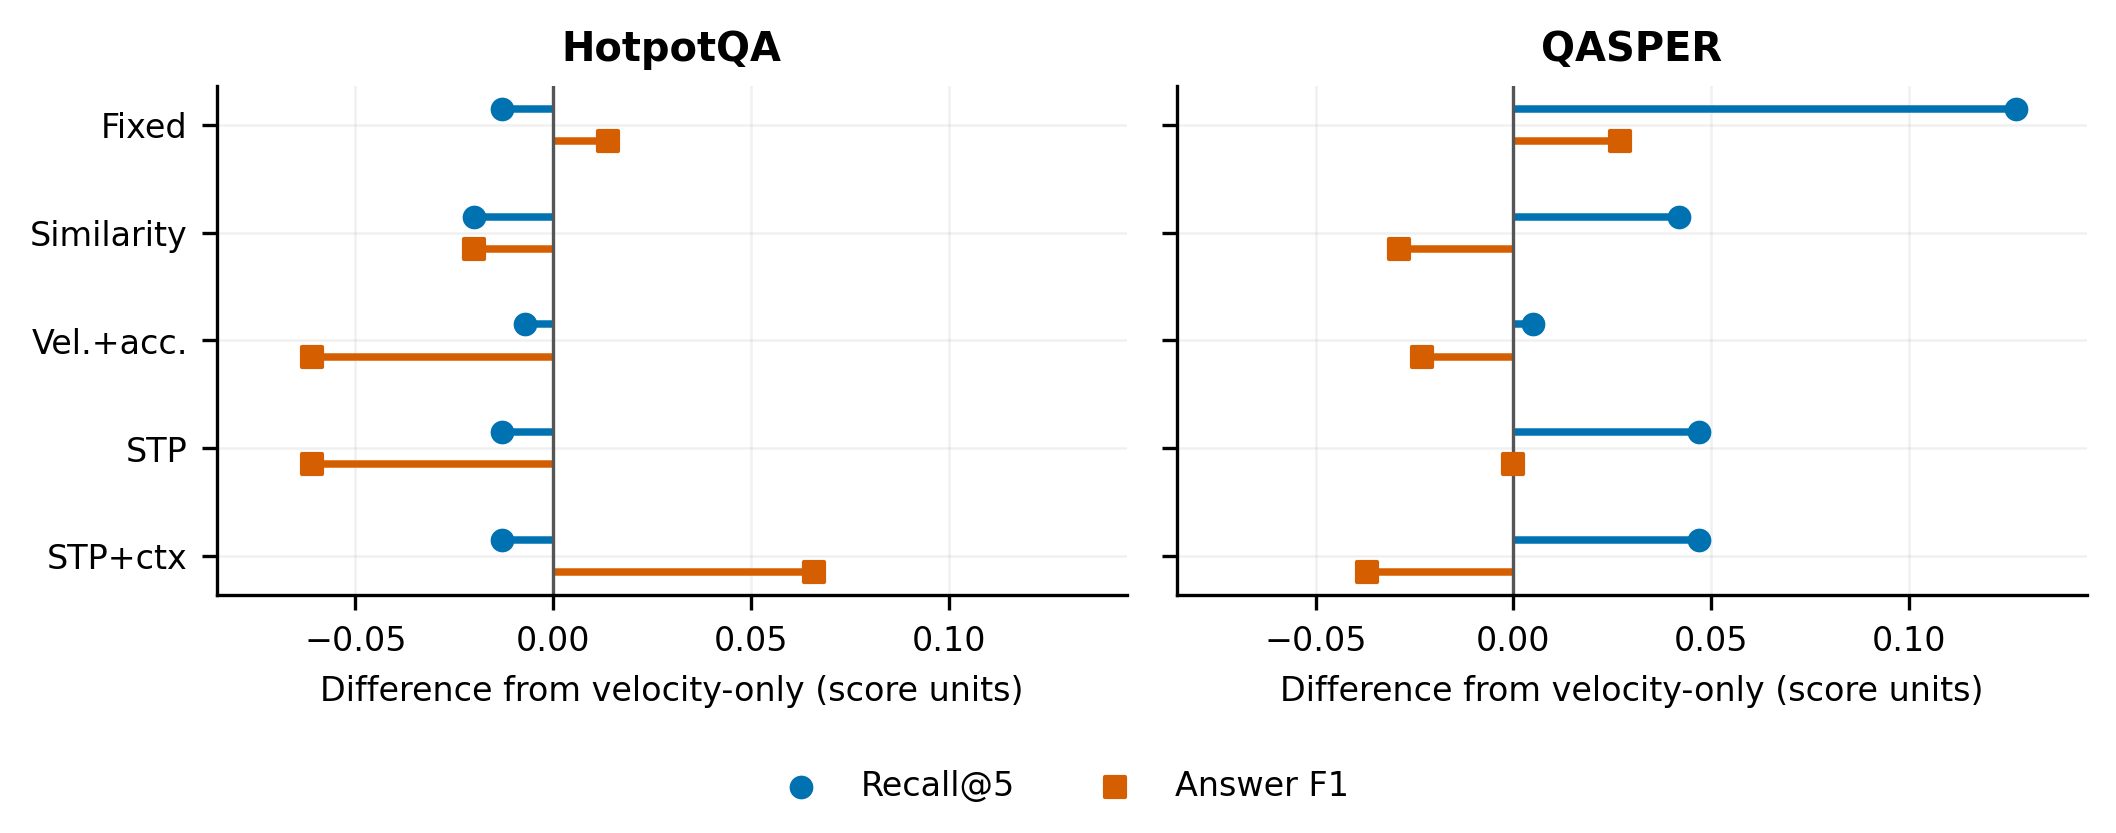
\includegraphics[width=\textwidth]{delta_vs_baseline.png}
\caption{Supplied rounded mean differences in Recall@5 and answer F1 relative to the nominal velocity-only arm, which includes structural weighting. Values are descriptive; plotted conditions without supporting ledger details are not verified comparisons.}
\label{fig:delta}
\end{figure}

\begin{figure}[t]
\centering
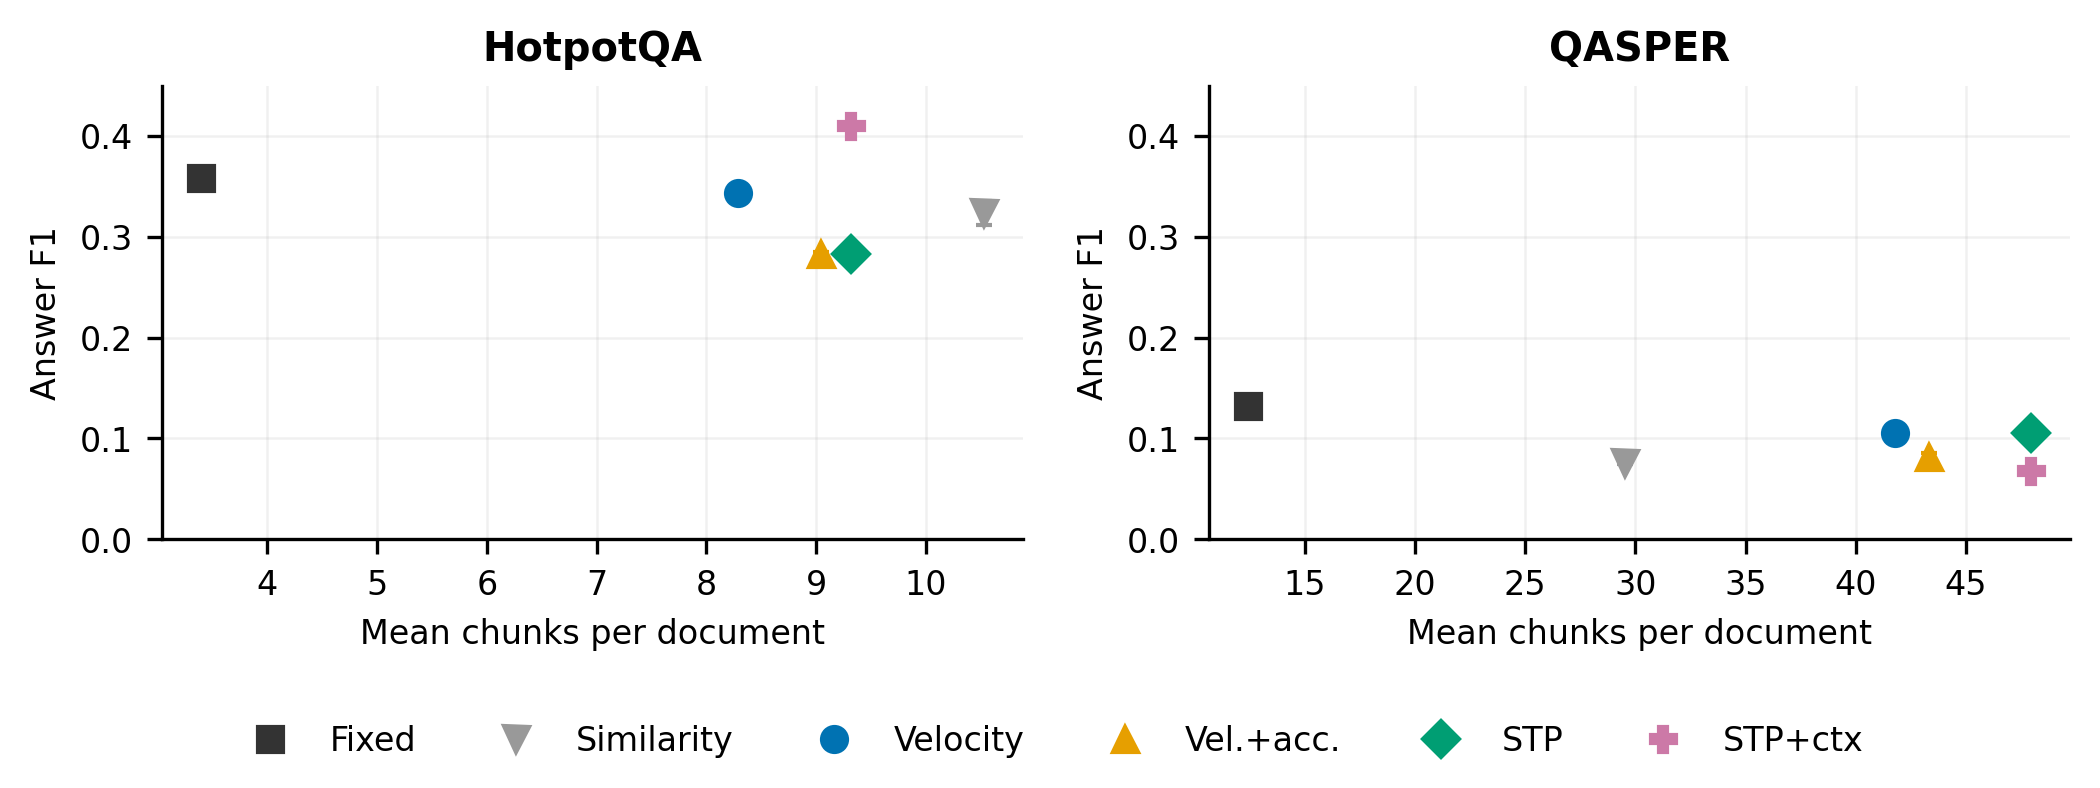
\includegraphics[width=\textwidth]{structure_breakdown.png}
\caption{Supplied descriptive plot of mean chunks per document against answer F1 by dataset and pilot label. Chunk counts do not establish section preservation, and plotted conditions without supporting ledger details are not verified comparisons.}
\label{fig:structure}
\end{figure}

\subsection{Confirmatory Evaluation Design}

The following protocol is unexecuted. It will use matched document and question splits across arms, matched chunk-length distributions, and matched generator prompt budgets. One JSONL row per query and arm will retain the query and document identifiers, retrieved and attached source spans, predictions, relevant metric inputs, and measured prompt tokens. Alignment losses and exclusions will be recorded so that the evaluated population is explicit.

The planned segmentation arms are fixed-size, similarity-threshold, clean velocity-only without structural cues, structure-only, velocity + volatility, velocity + structure, full STP without structure, and full STP. Relevance-only and profile-guided context are planned context-policy comparisons. These arms are intended to separate the contributions of transition features and structure from the effect of adding context; they are not completed ablations. Their exact configurations, length matching, context budgets, and comparison families must be specified before execution.

The evaluation will report Recall@K and MRR@10 for retrieval and exact match and answer F1 for generation. Before execution, it will fix the relevance mapping between source evidence and retrieved chunks, answer normalization, aggregation units, and handling of multiple evidence spans. Intrinsic segmentation evaluation will use $P_k$ and WindowDiff against reference boundaries, with the window size and reference treatment declared in advance. Operationally, evidence split rate will be the fraction of eligible reference evidence spans crossed by at least one chunk boundary. Context precision will be the fraction of attached context units overlapping reference evidence, and context recovery the fraction of eligible reference evidence units covered by attached context; overlap, deduplication, and zero-denominator handling will be fixed in advance. These measures distinguish evidence coverage from the amount of context supplied.

The protocol will also measure index size, index build time, retrieval latency, and prompt tokens, with hardware, backend, caching, timing boundaries, and aggregation procedures recorded. Paired bootstrap or document-cluster bootstrap intervals and a sign-flip permutation test are planned, with document clustering and comparison families specified before analysis. Holm correction will be applied to the prespecified family of hypothesis tests. These procedures and measures are plans, not pilot results.

\section{Limitations and Reproducibility}

\subsection{Interpretation Limits}

The generation evaluation comprises only 25 queries, and QASPER evidence alignment removes 42 of 149 questions. The retained set may differ from the original question set, and the available aggregates do not characterize the excluded questions. The nominal velocity-only arm includes structural weighting, while retrieval arms differ in indexed material and chunk counts. Generator evidence volumes and context attachment are also unmatched. Consequently, neither the component comparisons nor the context comparisons identify individual effects.

Aggregate means are available without released paired predictions, paired confidence intervals, or hypothesis tests. The mixed results do not establish causality or broad generalization. Retrieval timing is not end-to-end latency, and the discrepancy between the supplied timing figure and ledger further limits its interpretation. No deployment-speed claim follows.

\subsection{Reproducibility Gaps}

The available audit omits the encoder version, exact structural processing, calibrated weights, generator decoding, retrieval backend, hardware, and per-query records. It also does not fully specify the boundary and context-selection procedures needed to reconstruct the reference design. The planned query-arm JSONL records, configuration declarations, and budget controls are future remedies, not existing artifacts.

The supplied figures have been inspected and are included as descriptive assets. Their filenames and plotted labels do not establish additional numerical results, implementation details, or statistical evidence. Resolving the timing discrepancy and verifying the provenance and definitions of all plotted conditions require the underlying records.

\clearpage
\section{Conclusion}

STP-RAG specifies transition-based adaptive chunking and provenance-preserving selective context, and the audited pilot provides mixed descriptive observations rather than a confirmed improvement. HotpotQA answer F1 favors full STP with context in the reported aggregates, while QASPER favors fixed-size chunking and shows lower full-STP F1 with context. Small generation samples, alignment losses, and unmatched budgets constrain both findings. The next step is to execute the proposed matched-budget, paired protocol and verify the implementation and measurement records.

\bibliographystyle{plainnat}
\bibliography{references}
\end{document}